% RS comment and modifications 08/01/2014 


\documentclass[12pt,a4paper]{article}

\usepackage[T1]{fontenc}
\usepackage[latin9]{inputenc}
\usepackage{epsfig}
\usepackage{enumitem}
\usepackage{amsmath}
\usepackage{amsfonts}
\usepackage{lipsum}
\usepackage{titlesec}
\titlespacing\section{0pt}{12pt plus 1pt minus 1pt}{0pt plus 2pt minus 2pt}
\titlespacing\subsection{0pt}{5pt plus 1pt minus 1pt}{0pt plus 2pt minus 2pt}
\titlespacing\subsubsection{0pt}{5pt plus 1pt minus 1pt}{0pt plus 2pt minus 2pt}
%\usepackage[dcucite,abbr]{harvard}
%\harvardparenthesis{none}
%\harvardyearparenthesis{round}
%\newcommand{\citeasnoun}[1]{\cite{#1}}

%%%%%%%%%%%%%%%%%%%%%%%%%%%%%% User specified LaTeX commands.
%\usepackage{euler,times}
%\usepackage{euler,beton}	% RS comment out - normal text font

\usepackage[margin=1.3in]{geometry} % RS addition

% \newcommand{\footnoteremember}[2]{	% RS comment out - more simple affiliation
% \footnote{#2}
%   \newcounter{#1}
%   \setcounter{#1}{\value{footnote}}
% } 
% \newcommand{\footnoterecall}[1]{
% \footnotemark[\value{#1}]
% } 

\usepackage[authoryear]{natbib} % package to use Harwad style for reference http://www.andy-roberts.net/writing/latex/bibliographies

\begin{document}


\thispagestyle{empty}

  \vspace{-3cm}
  
\includegraphics[height=2cm]{./images/EPFL.pdf}
%  \hspace{1.5cm} \includegraphics[height=2cm]{./images/Trace.jpg} 
  \hfill 
\includegraphics[height=2cm]{./images/bestmile.jpg}
  
  \hrulefill
  \vspace{3.0cm}

%%%%%%%%%%%%%%%%%%%
%%  TITLE HERE  %%%
%%%%%%%%%%%%%%%%%%%
\begin{center}
 Master Project 
 \LARGE
 \bigskip
 
 Experimental Comparison of Autonomous Vehicles Routing Optimization Algorithms
\end{center}

%%%%%%%%%%%%%%%%%
%% TITLE HERE %%%
%%%%%%%%%%%%%%%%%


%%%%%%%%%%%%%%%%%%%
%% AUTHORS HERE %%%
%%%%%%%%%%%%%%%%%%%
\vspace{2.0cm}
\begin{tabbing}
\hspace*{3cm}		\=	\hspace*{5cm}							\=	\hspace*{3cm} \\
Author:			\>	Prisca Aeby		  \textsuperscript{1}	\> prisca.aeby@epfl.ch\\
Supervisors:		\>	Bastien Rojanawisut	  \textsuperscript{2}	\> bastien.rojanawisut@bestmile.com\\	
					\>	Boi Faltings    \textsuperscript{3}	\> boi.faltings@epfl.ch\\
\end{tabbing}
%%%%%%%%%%%%%%%%%%
% AUTHORS HERE %%%
%%%%%%%%%%%%%%%%%%



\begin{center}

\today
\end{center}

\vfill
\hrulefill

\small \textsuperscript{1} Computer Science,  \'Ecole Polytechnique F\'ed\'erale de Lausanne, Switzerland

\small \textsuperscript{2} Scala Backend Software Engineer, BestMile, Switzerland 

\small \textsuperscript{3} Artifical Intelligence Laboratory , School of Computer and Communication Sciences, \'Ecole Polytechnique F\'ed\'erale de Lausanne, Switzerland, \verb+liawww.epfl.ch+ 




\newpage


\begin{abstract}
Your abstract.
\end{abstract}

\newpage

\tableofcontents
\newpage
\setlength{\parskip}{0.5em}
\section{Introduction}
General problem: two types of services, on-demand and fixed-line => explain why we focus on fixed line (all constraints of the platform) 
Fixed line because now roads are not made for more complex systems


\section{Related Literature}
The scope of vehicle scheduling problems related to our specific case study can range from fixed-line bus services to on-demand systems. In fact, electric shuttles' routes and stops are predefined but timetables can be flexible to respond to the known real-time demand. The set of constraints differs from traditional bus transportation, for example workforce regulations can be eliminated as the shuttles are not human driven but a battery management component needs to be introduced into the planning process. As we will see in this chapter, current research often concentrates on one specific aspect of the scheduling strategy, simplifying some constraints, assessing the system's performance using various types of metrics and considering different inputs. In what follows, we describe in section \ref{pubtrans} some techniques used in the traditional public transport industry to guarantee a good quality of service. In section \ref{das} we describe the concept of Demand-Adaptive Transit Systems. Finally, we detail in section \ref{luts} an approach proposed by the Urban Transport Systems Laboratory at EPFL (LUTS) for scheduling autonomous vehicles activities.  

\subsection{Public Transport}\label{pubtrans}
Within the standard transit organization, policies and standards affect a lot the development of transport strategies and how people interact with the systems. The planning process of a fixed line bus transportation service is mainly composed of three different tasks: route planning, service frequencies and service timing. Route planning consists of defining a sequence of stops composing each route and how those routes are interconnected. Service frequency captures the number of vehicles per unit time which pass a given route (often expressed in vehicles per hour). A common measure used to express the ideal distance between vehicles is the headway, the inverse of the frequency, in other word the fixed interval at which vehicles are coming at a station. The service frequencies set by the transport organization can be chosen based on different policies (see \cite{tcrp}): 
\begin{enumerate}
\item \textbf{Fixed headway}: the agency establishes a fixed interval at which vehicles come to stations. It is convenient for customers as they have access to an exact schedule, but it is hard to keep the time between vehicles constant as it is vulnerable to external disturbances.
\item \textbf{Demand-based headway}: in existing transport services, agencies can adapt the timetables based on the observed demand at the stations (number of passenger boardings/deboardings) in order to reach the desired passenger load in vehicles.
\item \textbf{Performance-based headway}: the goal is to find the headway for which performance standards are optimized. Those costs are usually measured during a service period, for example a day. It may include the service productivity (e.g. the revenue per passenger per hour), the cost effectiveness of the service or the overall effectiveness (e.g. net subsidy per passenger). 
\end{enumerate}

All those scheduling strategies suffer from the well-known bunching effect: two or more buses arrive at the same time at a stop with the first one being overcrowded and the other one empty. This phenomenon occurs because of external disruptions in the service (e.g. stochastic passenger arrivals at stops, traffic jams, etc) (see \cite{hwadherence}) slowing down one of the bus which pick up passengers who would have taken the next bus. 

Several corrective measures based on different strategies have been developed to overcome this problem. There are mainly two different holding approaches to mitigate bus bunching as described in \cite{reliability}:

\begin{itemize}
\item \textbf{Headway-Based Holding:} vehicles arriving with a shorter headway at a stop (or holding point) wait to restore the headway distribution. If they arrive with a longer headway, it is possible to speed up the buses by skipping stations. The analytical study \cite{hybrid} proved the efficiency of using headway holding strategy and bus skipping (considering the extra waiting time of passenger whose station has been skipped) with the two-dimensional objective function composed of the regularization of bus headways on the one hand and the level of service with respect to a circle route scenario. 
\item \textbf{Schedule-Based Holding:} in the case of fixed timetables, schedule-based holding involves holding a vehicle at a stop if it is ahead of its schedule and dispatch it immediately otherwise.
\end{itemize}
  
\cite{selfadjusting} proposed a method using boarding limits at stations to control buses which does not involve bus accelerating or waiting at stations and thus does not influence the customers' travel time and does not disturb the traffic. They do not consider schedule and a priori target headway. However, they proved that their self-adjusting control stabilizes the headway spontaneously in a short time. 

\cite{loadFactor} study the importance of the vehicle load effects on the emission of vehicles through the study of the load factor and the empty running rate. The passenger load factor measures the efficiency of a transportation system, representing the capacity utilization of the seats. It is often expressed as the ratio between the passenger-kilometres travelled to seat-kilometres available. 

As stated by \cite{information}, the majority of earlier studies conducted on maintaining a balanced headway uses arrival time of the current bus at the current stop and arrival times of the preceding buses but does not take advantage of real time information like the vehicles' geolocation. Later methods proposed new approaches assuming availability of locations and even real-time arrivals of passengers to each bus stop. For example, \cite{cooperation} proposed a solution taking into account the distance between the current bus and the preceding and following buses to adjust the speed of the current bus. It includes holding buses at stations, accelerating or decelerating. 

The studies carried out within the traditional fixed-line bus services handle situations where the demand is consistently strong over the territory and where the fleet is composed of high-capacity vehicles. When the demand is weaker, it is complicated to operate an economical and frequent transit system as the resources are shared by few people and are very costly (e.g. driver salaries, fuel expenses, etc.). The autonomous fleets are composed of vehicles with lower capacity, but it is easier to dynamically adapt their scheduling strategy at low cost and have access to real-time information.

\subsection{Demand-Adaptive Transit Systems}\label{das}
Demand-Adaptive System (DAS), or Demand-Responsive Transit (DRT), is a personalized type of transportation displaying features from both fixed-line services and on-demand systems. In such systems, passengers are picked up and dropped off on-demand at predetermined stops, and unrequested stops are skipped. There are still compulsory stops, which are served within a predefined time window, but the routes are adapted based on the the requested stops. A method to determine the time windows at the compulsory stops has been proposed by  \cite{masterschedule}. \cite{dasdesign} depicted the advantages to substitute fixed-line bus services to DRT services in two cities in California with low demand density. 

\cite{evaluation} address the issues of evaluating DAS services in comparison to traditional transit services and fully on-demand systems. The transit systems' evaluation denotes the part of the planning process dedicated to the study of the behaviour and the performance of the line under various conditions with respect to demands, policies and costs. They mention the main steps of transit lines' evaluation in order to tune operating parameters impacting the system performance under different scenarios for cost-benefit analyzes: 1) the scenario, parameters and policies are specified, as well as the demand to serve 2) the line is designed 3) the operation of the line is simulated (during a specified time-horizon) 4) results are collected and performance measures are computed. The importance of demand generation in step 1) differs from one system to the other: whilst in fixed lines transits static methods are often used to simulate an average demand, dynamic methods are used to simulate the time-dependent stop-to-stop requests in on-demand systems. The performance measurements in step 4) vary as well from one system to the other: in fixed-lines the service quality is mainly represented by the buses' punctuality and the constant interarrival times whereas for on-demand systems it is expressed by the specific users' waiting time and journey time. \cite{evaluation} propose a framework for evaluating DAS lines including the scenario input, the optimization modules for the design and operation of the line and the simulation module which yield the statistical information about the performance.

\subsection{Vehicles Assignment to Routes}\label{luts}
\cite{luts} present an optimization approach for the autonomous vehicles scheduling within a transit system composed of circular routes. They separate the planning process in two main tasks: line planning and vehicle scheduling. Line planning corresponds to defining the routes and the required headway on each route over the planning horizon. Vehicle scheduling refers to computing a general assignment plan for each vehicle for each time period over the planning horizon of one day. It means that each vehicle is assigned to a specific route or to a recharging station for each time period. The underlying assumption is that the vehicles will not transfer between routes and charging stations too often which makes the time discretization of the planning horizon possible. They focus on the vehicle scheduling task which takes as input the predefined routes, frequencies, fleet size and battery model. They present the scheduling problem as a mixed-integer linear programming (MILP) with battery constraints and the goal of the objective function being to maximize the total battery charge levels at the end of the planning horizon. 

\section{Problem Formulation}
In this section we formulate the mathematical model describing the autonomous vehicles circular line system. All the variables are listed in Table \ref{table:parameters}. In addition to traditional bus transit system descriptions, we introduce the concept of battery stations and we include dynamic bookings from one station to an other station on the loop. As we have access to information during the service horizon time $H$, we denote a discrete timestamp $t$ which takes values between $[0, H]$ at fixed sampling $interval$.
\begin{table}
\makebox[\textwidth][c]{
  \centering
\begin{tabular}{| l | l |}
  \hline			
  & Signification \\
  \hline		
  $S = \{1,..., n\}$ & Set of stations on the route \\
  $E =  \{n+i,..., 2n\}$ & Set of directed edges linking the stations \\
  $V = \{1,..., v\}$ & Set of vehicles composing the fleet \\
  $C \subset S$ & Set of charging locations \\
  $B = \{1,... b\}$ & Set of bookings made during the scheduling horizon \\
  $B^{*} \subset B$ & Set of bookings which have been satisfied at the end of $H$\\
  
  $H$ & Length of the scheduling horizon \\
  $interval \in \mathbb{R}$ & Interval at which values are sampled \\
  $T = \{t = interval * k, k \in \mathbb{N} | 0 < t < H\}$ & Set of timestamps  \\
  $c^{v}$ & Maximum load capacity of vehicle $v \in V$\\
  $q^{v}$ & Maximum charge of vehicle $v \in V$\\
  $\alpha^{v}$ & Battery recharge rate of vehicle $v \in V$\\
  $\beta^{v}$ & Battery consumption rate of vehicle $v \in V$\\
  $s^{v}$ & Maximum speed of vehicle $v \in V$ \\
  
  $speed^{e}_{t}$ & Speed of edge $e$ at time $t$ \\
  $I^{v}_{t} \in [0, q^{v}]$ & Battery level of vehicle $v$ at time $t$ \\  
  $\delta^{v}_{t}$ & Battery change between $t$ and its preceding timestamp \\  
  $e^{v}_{t}$ & Edge $e \in E$ which vehicle $v$ is traversing at time $t$ \\
  $next^{v}_{t}$ &  Distance to the next vehicle in front of $v$ on the loop at time $t$ \\
  $o^{v}_{t} \in [0, c^{v}]$ & Number of passengers in vehicle $v$ at time $t$ \\
  $i^{v}_{t}$ & Seconds vehicle $v$ needs to stop at time $t$ \\  
  
  $b_{i,j} \in B$ & Request of trip from station $i$ to station $j$, $i,j \in S$ \\
  $t^{b}$ & Time at which the request $b \in B$ has been made \\
  $n^{b}$ & Number of passengers for booking $b \in B$ \\
  $p^{b}$ & Pick-up timestamp of booking $b$ \\
  $d^{b}$ & Drop-off timestamp of booking $b$ \\
  $w^{b}$ & Waiting time of booking $b$ \\
  $\Delta^{b}$ & Journey time of booking $b$ \\
  
  $A^{s}, s \in C$ & 1 if $s$ is an available charging station, 0 otherwise \\
  $M^{s}$ & 1 if $s$ is the stop is mandatory, 0 otherwise \\
  $x^{v}_{t}$ & 1 if the vehicle $v$ is charging at a station at time $t$, 0 otherwise \\
  $D_{b}$ & 1 if request $b$ has been satisfied \\
  \hline  
\end{tabular}
}
\caption{Problem sets and parameters}
\label{table:parameters}
\end{table}
\subsection{Circular Route}
The circular line in this transportation system is a route which starts at a certain station, traverses other stations once and terminates at the starting station. The route is represented by set of stations  and a set of directed edges $E$ linking each station $s \in S$ to its following station. The set of charging stations $C$ includes stations located on the stops within the loop: $C \subset S$. If the charging station is not used by any vehicle of the fleet we have $A^{s} = 1$. A stop $s$ can be mandatory (vehicles always stop when they reach the stop) or optional (the stop can be skipped). If the stop is mandatory the boolean variable $M^{s}$ is set to 1, and 0 otherwise. The maximum speed of an edge, representing the traffic at time $t$, is expressed as $speed^{e}_{t}$.

\subsection{Vehicles}\label{vehicles}
Each vehicle composing the fleet $v \in V$ moving on the circular closed line is characterized by a capacity $c^{v}$, a maximum charge $q^{v}$, a recharge rate $\alpha^{v}$, a battery consumption rate $\beta^{v}$ and a maximum speed $s^{v}$. The battery level of vehicle $v$ at the timestamp $t$ is $I^{v}_{t} \in [0, q^{v}]$. The battery change between the preceding discrete timestamp and the current timestamp $t$ is given by $\delta^{v}_{t}$. The edge it is currently traversing is $e^{v}_{t}$ and the distance to the next vehicle in front of it on the loop is given by $next^{v}_{t}$. The occupancy of the vehicle is expressed as $o^{v}_{t} \in [0, c^{v}]$. The vehicle is travelling either at its maximum speed or at the limitation of the current edge. Its current speed is therefore max$\{s^{v}, speed^{e^{v}_{t}}\}$. When a vehicle is charging at a station the boolean variable $x^{v}_{t}$ is set to 1 and it can not carry any passengers $o^{v}_{t} = 0$. A vehicle entering a station at time $t$ might have to wait $p^{v}_{t}$ seconds.

\subsection{Bookings}\label{bookings}
The set $B$ represents the users' bookings made during the service horizon. A booking $b_{i,j} \in B$ requests a trip from station $i$ to $j$ at time $t^{b}$ for a group of $n^{b}$ persons. If the booking has been satisfied, the boolean variable $D_{b}$ is set to 1 and we know that it has been executed by vehicle $v^{b} \in V$. The pickup time of booking $b$ at station $i$ is $p^{b}$ and drop-off time at station $j$ is $d^{b}$. The waiting time  $w^{b}$ equals $p^{b} - t^{b}$ and the journey time $\Delta^{b}$ is $d^{b} - p^{b}$. We denote $B^{*}$ the set of bookings which have been satisfied, so the bookings for which $D_{b} = 1$.

\subsection{Output Metrics}\label{metrics}
At the end of the service horizon $T$, some metrics can be derived in order to evaluate the performance of the overall system dispatching the vehicles to serve the requests. 

\subsubsection*{Battery}
The total battery consumed by a vehicle $v$ is the sum of the battery changes over the scheduling horizon when the vehicle is not charging:
$$battery^{v} = \sum_{t \in T}\delta^{v}_{t} * (1-x^{v}_{t}) $$
The total battery cost for the entire system is therefore the sum of the battery consumption of each vehicle composing the fleet:
$$batteryCost = \sum_{v \in V}battery^{v}$$
\subsubsection*{Occupancy}
The average occupancy of a vehicle $v$ over the scheduling horizon $T$ is given by:
$$avgOccupancy = \frac{\sum_{t \in T}o^{v}_{t}}{|T|}$$
The average occupancy does not take into account of the time vehicles spend at charging stations and therefore can not carry any passenger. As explained in section \ref{pubtrans}, a common unit used in transportation  measurement is the load factor, which expresses the efficiency of a vehicle based on the kilometres travelled by passengers over the total kilometres that could have been driven considering its maximum capacity. In our case, as we are mainly interested in how the battery of the vehicles has efficiently been used, we define the passenger-battery measure: it is the battery that has been consumed by the vehicle during the passenger journey time. The passenger-battery for one vehicle is therefore the sum of the passenger-battery of the bookings it has satisfied. The seat-battery available represents the maximum possible passenger-battery if the vehicle would have been always full: it is the battery consumption of the vehicle times its maximum capacity. The vehicles' load factor is its passenger-battery over its seat-battery:
$$loadFactor^{v} = \frac{\sum_{t \in T} \delta^{v}_{t} * (1-x^{v}_{t}) * o^{v}_{t}}{battery^{v} * c^{v}}$$
We can compute the average load factor of the fleet as:
$$avgLoadFactor = \frac{\sum_{v \in V}loadFactor^{v}}{|V|}$$
We denote the stability load factor the difference between the maximum load factor among the vehicles composing the fleet and the minimum one. The closer it is to 0 the better as it implies that all vehicles are used equivalently: $stabilityLoadFactor = \max_{v^{+} \in V}{loadFactor^{v^{+}}} -  \min_{v^{-} \in V}{loadFactor^{v^{-}}}$.
\subsubsection*{Waiting Time}
The average waiting time among the satisfied bookings is given by: 
$$avgWaitingTime = \frac{\sum_{b \in B{*}}w^{b}}{|B^{*}|} $$
The stability waiting time is the difference between the maximum waiting time and the minimum waiting time among the bookings:  $stabilityWaitingTime = \max_{b^{+} \in B^{*}}{w^{b^{+}}} -  \min_{b^{-} \in B^{*}}{w^{b^{-}}}$.
\subsubsection*{Journey Time}
The average journey time among the satisfied bookings is given by:
$$avgJourneyTime = \frac{\sum_{b \in B^{*}}\Delta^{b}}{|B^{*}|} $$

\subsubsection*{Completed Bookings Percentage}
Travel time, booking time, 
At the end of the scheduling horizon, some bookings may not have been satisfied. The percentage of bookings which have been satisfied is given by:
$$completedBookings = \frac{|B^{*}|}{|B|}$$

\section{Methodology}
In order to evaluate the behaviour and performance of the system under various conditions with respect to the line configurations, the booking scenarios and the vehicles scheduling alternatives, we undertake analyses under laboratory conditions by simulating the operation of the system on the platform dispatching the vehicles. One of our main goal in the analysis we conduct on the line is to get measures as close as possible to real world conditions. In order to achieve this, a dynamic system is required which handles the time-dependent events of the system. In section \ref{framework} we describe the behaviour of the different interconnected services simulating the vehicles' behaviour reacting to external conditions and how the overall system is evaluated. In section \ref{scheduling} we present the variations of scheduling strategies used to dispatch the vehicles on the line. The parameters characterizing the simulation framework and the ones introduced in the scheduling strategy are summarised in table \ref{table:simparameters}. 

\subsection{Simulation Framework}\label{framework}
\setlength{\belowcaptionskip}{10pt}
\begin{figure}[h] 
  \centering
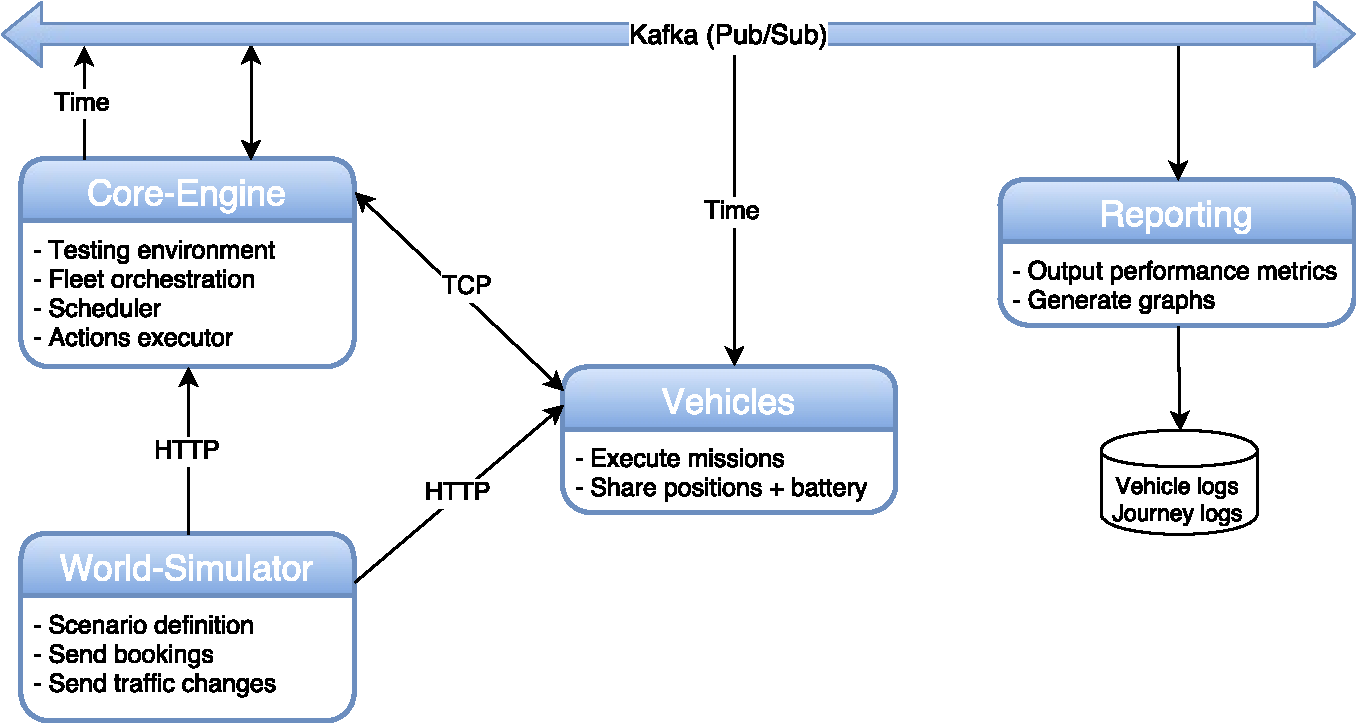
\includegraphics[scale=0.55]{./images/SimulationFramework2.pdf}
\caption{Interconnected modules composing the simulation framework}
\label{fig:simulationFramework}
\end{figure}

Figure~\ref{fig:simulationFramework} illustrates the different web services and how they are linked to each others. Services can communicate by exchanging messages via Kafka which is an asynchronous publish-and-subscribe message broker. In what follows we describe the behaviour of each module and the simulation parameters which can be tuned. 

\subsubsection{World-Simulator}
The world-simulator is a web service which is used to start the simulation, send the booking requests and send traffic updates information through the HTTP connection established with the core-engine application. At the beginning of the simulation, it sets the time control to a given ratio which is sent to the core-engine application.  A day can be simulated in $m$ minutes which corresponds to a ratio $r$ of $m / 24h$. The simulated time $simTime$ is therefore $r$ times the real time. The world-simulator is instantiated with a scenario describing the external events which affect the overall system. It mimics the bookings which would have been made by users with the booking application and sent through a REST API. Every second at time $simTime$ it checks if there are bookings with $t^{b} = simTime$ and speed updates to send to the core-engine application with $speed_{t}^{e}, t = simTime$. 

\subsubsection{Simulated Vehicles}
Vehicles are connected to the core-engine through an established TCP protocol. They can send status messages and receive missions, like going to a specific charging station or waiting at a stop at for $p^{v}_{simTime}$ seconds. A vehicle executes every mission it receives from the core-engine. The vehicles are simulated concurrently following an actor model. Each vehicle is a different actor part of the actor system. When the vehicles web service receives an HTTP request to start the simulation with a given fleet size from the world-simulator, an actor is created for each vehicle, which announces its position to the core-engine through a TCP message and subscribes to the time topic. The vehicles start at equal distance of each others on the loop with the battery completely recharged and their position and battery level is then updated every $1000/rate$ milliseconds.  

\subsubsection{Core-Engine}
The core-engine application is a distributed system that combines and processes real-time information for coordinating and optimizing the fleet of autonomous vehicles. Several testing environment components are instantiated by the core-engine application: the map, the vehicles' configurations and fleet schedule through the day. The map is a GeoJSON file which is translated into the application to a directed graph with an edge between every stop and charging stations. The vehicles' configurations include all the parameters enumerated in section \ref{vehicles}. The core-engine handles the bookings it receives from the world-simulator, updates the edges' speed of the graph and sends the actions to be executed by the vehicles. When it receives the starting simulation time and ratio $r$ from the world-simulator, it publishes the updated time to the corresponding Kafka topic. The scheduler component manages the number of vehicles which need to be on service at different times during the day and sends corresponding missions to the vehicles. The positions and battery states received from the vehicles through the TCP connection are then published to the corresponding Kafka topics.  

\subsubsection{Reported Metrics}
The reporting web-service subscribes to the vehicle and journey topics and writes the stream events to its database. An event for vehicle $v$ at time $t$ includes its speed, position, battery level and battery state $x_{t}^{v}$. There is an event only for a booking which has been satisfied $b \in B^{*}$ and it includes all the parameters listed in section \ref{bookings}. At the end of the simulation, events are fetched from the database at fixed sampling $interval$ and then those logs are analysed in order to compare different scenarios in term of their overall performance. All the metrics listed in section \ref{metrics}. In addition, we represent visually the simulation's performances with different graphs. In order to evaluate the different behaviours among the vehicles, we plot the hourly average occupancy of each vehicle during the scheduling horizon $H$. It is useful to see if all the vehicles are carrying passengers through the scheduling period or only few of them. We compare as well the number of vehicles which are at charging stations to the hourly average waiting time. It gives a good indicator to determine if the time at which the vehicle has been sent to charge was appropriate or if it impacts a lot the service in terms of quality of service provided to the passengers.

\subsection{Scheduling}\label{scheduling}
The approach proposed by \cite{luts} described in section \ref{luts} is formulated as an optimization problem which considers the optimal headway for each route as an input but does not specify how to define it. Many real world aspects are not considered in their model. For example, it does not include transfers costs to charging stations or the time it takes to stop at stations and board passengers. It does not evaluate any demand scenarios neither. Our approach is to focus on scenarios as close as possible to real world conditions and find heuristics to define the number of vehicles needed on the fixed line in order to have a good balance between the battery consumption and the quality of service offered to the passengers. In what follows we describe how the core-engine handles the missions it sends to the vehicles based on the dynamic events it receives. 

\subsubsection{Vehicles' Activities Schedule}\label{schedule}
When a vehicle $v$ arrives at a station $j$ at $simTime$, it checks if it is carrying passengers which have made a booking $b_{i,j}$. If it is the case it needs to stop and its load is updated. If any booking $b_{j,k}$ has not been picked up yet $b \not\in B^{*}$ and that the condition $o^{v}_{simTime} + n^{b_{j,k}} \leq c^{v}$ holds then it picks up the passenger(s) from the booking request. It waits $i^{v}_{simTime}$ seconds based on the headway computation which is explained in section \ref{hw}. If the vehicle does not need to stop to drop off or pick up passengers and that the station $s$ is not mandatory $M^{s} = 0$ then it can simply skip the station.   

The battery level $I^{v}_{simTime}$ of vehicle $v$ is controlled every time a vehicle arrives at a station. If it is under a threshold $minBatt$, it can not pick up any passenger any more, need to drop off every passenger at their requested drop-off station and finally goes the the closest charging station. When a vehicle is recharging and there is a booking $b$ not picked up yet, $D_{b} = 0$, then the vehicle is dispatched on the loop again if its battery level is above a threshold denoted $enoughBatt$. 

\subsubsection{Headway}\label{hw}
Even though the vehicles start at equal distance at the beginning of the scheduling horizon, if no strategy is adopted to maintain an equal distance between them the system will suffer from the well-known bus bunching effect described in section \ref{pubtrans}. In fact, the buses picking up passengers (which need to wait longer at stations) are slowing down and their preceding buses will catch them up, especially if some stations are not mandatory and they can skip them. As we have at our disposal updated vehicles' states, we can adopt a decentralized strategy in order to dynamically balance the distances between the active vehicles operating on the loop. The idea is to compute the ideal distance between the vehicles and to stop longer the ones too close to their following vehicle on the line, or on the other hand stop less if they are too far. As explained in section \ref{schedule}, each time a vehicle stops at a station we compute the number of seconds it has to wait until it can leave. We set a default 

\subsubsection{Dynamic Fleet Size}
how choose vehicles to send to charge and which ones to activate

\begin{table}9
\makebox[\textwidth][c]{
  \centering
\begin{tabular}{| l | l |}
  \hline			
  & Signification \\
\hline	  
  $r$ & Simulation ratio: simulated time = $r$ times real time\\
  $simTime$ & Current simulated time on the different applications \\
  $rate$ & Rate at which vehicles' state is updated \\
  $interval$ & Interval at which events are fetched from the reporting database \\
  $minBatt$ & A vehicle $v$ needs to finish its mission(s) and go to charge if $I^{v}_{t} < minBatt$\\
  $enoughBatt$ & A vehicle $v$, $x^{v}_{t}$, can leave the charging station if $I^{v}_{t} < minBatt$\\
  \hline  
\end{tabular}
}
\caption{Simulation framework and scheduling parameters}
\label{table:simparameters}
\end{table}




\section{Numerical Experiments}
Real environment
\subsection{Simulation Settings}
tuning
speed of actors
logs fetched from db

\subsection{Graph}
Unless stated, charging locations at same place
\subsection{Optimal Headway}
\subsection{}

\subsection{Simulated Demand}
\subsection{}

\section{Conclusion}

\bibliographystyle{apalike}
\bibliography{/Users/prisca/Documents/Final_Report/bibliography/bibliography}

\end{document}
